\chapter{Tratamiento inicial de los datos: análisis descriptivo}
\label{chap:tratamiento_inicial_de_los_datos}

\section{Descripci\'on de los datos}


\begin{wrapfigure}[17]{R}{0.5\textwidth}

\includegraphics[width=0.45\textwidth]{tuit_ejemplo}
\caption{Ejemplo de tuit.}\label{fig:tuit_ejemplo}
\end{wrapfigure} 


En pantalla, un tuit relevante para nuestro proyecto podría ser el 
mostrado en la figura ad\-ya\-cente. Sin embargo, cuando descargamos el mismo tuit a través del API Search de Twitter, 
obtenemos mucha más información, en formato JSON. 

El formato JSON ({\em Javascript Object Notation})\footnote{\url{http://www.json.org/json-es.html}} 
es un formato ligero de intercambio de datos, fácilmente interpretable (por humanos y por
máquinas). Es un formato ampliamente utilizado, siendo numerosos los
lenguajes que son capaces de usar este formato (lenguajes de la familia C,Javascript, PHP, Python, etc.). 
En JSON se pueden representar dos tipos
de estructuras: un conjunto de pares (clave,valor) con la sintaxis \{clave1:valor1, clave2:valor2,\dots\}, también
denominado {\em objeto}, y un conjunto ordenado de valores con la sintaxis [valor1, valor 2,\dots] (que se denomina {\em arreglo}). 
Un valor puede ser una cadena de caracteres con comillas dobles, un número, un valor booleano o nulo, 
un objeto o un arreglo. Esta flexibilidad permite representar datos de gran complejidad.

Como veremos en el siguiente ejemplo de un tuit en formato JSON descargado a través del API Search de Twitter,
puede resultar de ayuda pensar en un JSON como en un diccionario \{clave:valor\}, donde las claves
son cadenas de texto, y el valor es algo flexible que acomoda desde una cadena de texto a un vector de objetos 
o un nuevo diccionario. En particular, la información del tuit que considerábamos más arriba 
luce de la siguiente manera:

\bigskip


\{'\_id': ObjectId('59e0cbb03842ed08188233d7'),

\quad'contributors': None,

\quad'coordinates': None,

\quad'created\_at': 'Wed Oct 11 08:13:41 +0000 2017',

\quad'entities': \{'hashtags': [\{'indices': [90, 106],'text': 'MachineLearning'\},

				  \hspace{4cm}\{'indices': [107, 114],'text': 'Python'\}],

	\hspace{2cm} 'symbols': [],

	\hspace{2cm}'urls': [\{'display\_url': 'twitter.com/i/web/status/9…',

				\hspace{3cm}'expanded\_url': 'https://twitter.com/i/web/status/918026805080182785',

				\hspace{3cm}'indices': [116, 139],

				\hspace{3cm}'url': 'https://t.co/1WuwNRzn8z'\}],

	\hspace{2cm}'user\_mentions': []\},

\quad'favorite\_count': 1,

\quad'favorited': False,

\quad'geo': None,

\quad'id': 918026805080182785,

\quad'id\_str': '918026805080182785',

\quad'in\_reply\_to\_screen\_name': None,

\quad'in\_reply\_to\_status\_id': None,

\quad'in\_reply\_to\_status\_id\_str': None,

\quad'in\_reply\_to\_user\_id': None,

\quad'in\_reply\_to\_user\_id\_str': None,

\quad'is\_quote\_status': False,

\quad'lang': 'es',

\quad'metadata': \{'iso\_language\_code': 'es',

	 \hspace{2.3cm}'result\_type': 'recent'\},

\quad'place': None,

\quad'possibly\_sensitive': False,

\quad'retweet\_count': 0,

\quad'retweeted': False,

\quad'source': '\verb|<a href="http://twitter.com"  rel="nofollow">Twitter Web Client</a>|',

\quad'text': 'Vamos preparando el siguiente libro a estudiar que al final la movida 

\hspace{1.7cm}me está gustando... \#MachineLearning \#Python… https://t.co/1WuwNRzn8z',

\quad'truncated': True,

\quad'user': \{'contributors\_enabled': False,

\hspace{1.7cm}'created\_at': 'Sat Dec 12 09:13:46 +0000 2009',

\hspace{1.7cm}'default\_profile': False,

\hspace{1.7cm}'default\_profile\_image': False,

\hspace{1.7cm}'description': 'Me gustan las camisetas y las  zapatillas // Desarrollo y '

\hspace{3cm}'Diseño para sistemas Apple //  Creador de @GetPomodoroApp ·  '

\hspace{3cm}'@GetAtentoApp · @MADatBUS ·  @GetMeteo y...',

\hspace{1.7cm}'entities': \{'description': \{'urls': []\},

\hspace{3.5cm}'url': \{'urls': [\{'display\_url': 'desappstre.com',

\hspace{4.5cm}'expanded\_url': 'http://desappstre.com',

\hspace{4.5cm}'indices': [0,23],

\hspace{4.5cm}'url': 'https://t.co/oYY42NlHrT'\}]\}\},

\hspace{1.7cm}'favourites\_count': 1512,

\hspace{1.7cm}'follow\_request\_sent': False,

\hspace{1.7cm}'followers\_count': 211,

\hspace{1.7cm}'following': False,

\hspace{1.7cm}'friends\_count': 209,

\hspace{1.7cm}'geo\_enabled': True,

\hspace{1.7cm}'has\_extended\_profile': True,

\hspace{1.7cm}'id': 96309647,

\hspace{1.7cm}'id\_str': '96309647',

\hspace{1.7cm}'is\_translation\_enabled': False,

\hspace{1.7cm}'is\_translator': False,

\hspace{1.7cm}'lang': 'es',

\hspace{1.7cm}'listed\_count': 109,

\hspace{1.7cm}'location': 'Madrid — Mundo Real™',

\hspace{1.7cm}'name': 'Adolfo ™',

\hspace{1.7cm}'notifications': False,

\hspace{1.7cm}'profile\_background\_color': '000000',

\hspace{1.7cm}'profile\_background\_image\_url': 'http://abs.twimg.com/images/themes/theme2/bg.gif',

\hspace{1.7cm}'profile\_background\_image\_url\_https': 'https://abs.twimg.com/images/themes/theme2/bg.gif',

\hspace{1.7cm}'profile\_background\_tile': False,

\hspace{1.7cm}'profile\_banner\_url': 'https://pbs.twimg.com/profile\_banners/96309647/1501577205',

\hspace{1.7cm}'profile\_image\_url': 'http://pbs.twimg.com/profile\_images/888396793024794624/O6gHh-lJ\_normal.jpg',

\hspace{1.7cm}'profile\_image\_url\_https': 'https://pbs.twimg.com/profile\_images/888396793024794624/O6gHh-lJ\_normal.jpg',

\hspace{1.7cm}'profile\_link\_color': '1B95E0',

\hspace{1.7cm}'profile\_sidebar\_border\_color': '000000',

\hspace{1.7cm}'profile\_sidebar\_fill\_color': '000000',

\hspace{1.7cm}'profile\_text\_color': '000000',

\hspace{1.7cm}'profile\_use\_background\_image': False,

\hspace{1.7cm}'protected': False,

\hspace{1.7cm}'screen\_name': 'FitoMAD',

\hspace{1.7cm}'statuses\_count': 6893,

\hspace{1.7cm}'time\_zone': 'Madrid',

\hspace{1.7cm}'translator\_type': 'none',

\hspace{1.7cm}'url': 'https://t.co/oYY42NlHrT',

\hspace{1.7cm}'utc\_offset': 7200,

\hspace{1.7cm}'verified': False\}\}

\bigskip

La descripción de cada campo de los que integran el tuit puede encontarse en la página web de Twitter para 
desarrolladores, \url{https://developer.twitter.com/en/docs/tweets/data-dictionary/overview/tweet-object}.

\section{Obtenci\'on de los datos}
Los tuits que componen nuestro corpus de datos los hemos obtenido a través del API Streaming
de Twitter, a través de una búsqueda dirigida en el API Streaming. Esta búsqueda dirigida 
se ha realizado a través de palabras clave, asociadas a la actividad de data science, concretamente:

\begin{center}
\begin{tabular}{ccccc}
\lq\lq machine learning\rq\rq  &\lq\lq machinelearning\rq\rq  &\lq\lq datamining\rq\rq  &\lq\lq data mining\rq\rq 
&\lq\lq Python\rq\rq\\
\lq\lq SQL\rq\rq & \lq\lq hadoop\rq\rq  &\lq\lq bigdata\rq\rq  &\lq\lq big data\rq\rq  &\lq\lq pentaho\rq\rq\\
\lq\lq rstats\rq\rq &\lq\lq SAS\rq\rq &\lq\lq tableau\rq\rq
\end{tabular}
\end{center}

Esta petición se define como un vector en Python, donde la coma significa \lq\lq OR\rq\rq y el espacio
dentro de las comillas significa \lq\lq AND\rq\rq, y se incluyeron dichos términos con y sin almohadilla 
(\#).

También hemos incluido en la búsqueda un filtro por idioma, incluyendo el parámetro 
\lq\lq languages = ["es"]\rq\rq en la llamada al API, con el objetivo de bajar solo tuits
en un idioma. En principio\footnote{\url{https://developer.twitter.com/en/docs/tweets/filter-realtime/guides/basic-stream-parameters }}
esta búsqueda debería devolver tuits que la aplicación Twitter ha detectado como escritos en
idioma español. Sin embargo, también bajamos tuits en otros idiomas (inglés, sobre todo), lo que
nos obligará a incluir esta variable en el proceso de selección de usuarios, como veremos en la sección \ref{sect:limpieza_de_los_datos}.

El script en el que se realiza la llamada al API de Twitter y el primer almacenamiento de los tuits
es el script llamado {\bf download\_tweets\_stream.py}. Este script importa otros
denuestro proyecto, como {\bf OpenMongoDB.py}, que gestiona la conexión a la base de datos MongoDB
en el que se almacenarán los tuits. El lanzamiento programado de la tarea se hizo con una entrada en el gestor
de Tareas Programadas del portátil, a través del archivo {\bf streaming\_upload.bat}. Todos estos
archivos se encuentran en el repositorio de GitHub descrito en la sección \ref{sect:repositorio}.


\section{Almacenamiento}
Según van produciéndose los tuits, y nuestra \lq\lq grabadora\rq\rq los va detectando, los hemos almacenado
en una base de datos de MongoDB, en local.


\section{Revisión inicial de los datos}
Una vez almacenados los tuits, realizamos un análisis exploratorio para estudiar con qué material contábamos para el desarrollo del proyecto. Este estudio se lleva a cabo en el archivo {\bf analisis\_exploratotio.py} del repositorio de
GitHub.

\subsubsection{Tuits repetidos}
Aunque hemos usado una conexión con el API Streaming de Twitter, que va almacenando los
tuits según van publicándose,  de los $14.736$ documentos que hemos recogido en la base de datos, 
solo $14.727$ son únicos, y hay $9$ repetidos. Esto es extraño, pero podría deberse a dos procesos
de Streaming corriendo en paralelo sobre la misma base de datos momentáneamente. Como son muy pocos, no los hemos eliminado para hacer este estudio previo de los datos.

\subsubsection{El texto de los tuits}
Nuestra primera duda es si los tuits que hemos bajado corresponden realmente a contenido relacionado
con la ciencia de datos. Esto será objeto de una sección propia a la hora de limpiar los datos.
De momento, una forma gráfica de ver si los textos de los tuits se corresponden con el tema
que nos interesa es construir una nube de palabras con dichos textos. Aparentemente no hay grandes desviaciones del tema a tratar, ciencia de datos y big data:

\myfigure{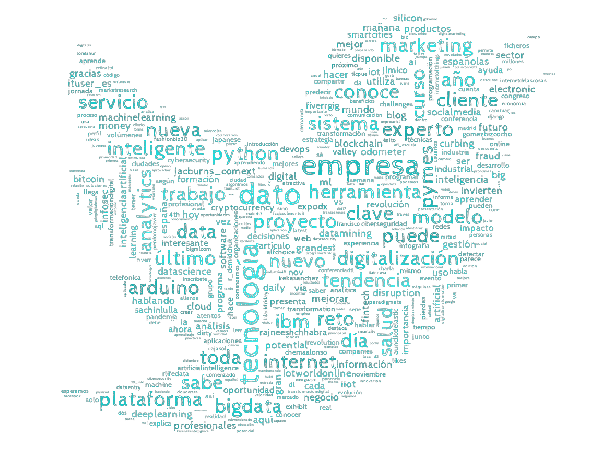
\includegraphics[scale = 1.15]{C:/DATOS/MBIT/Proyecto/MBITProject_Data4all/Python/images/twitter_worldcloud.png}%
\figcaption{Texto de los tuits}
\label{fig:twitter_worldcloud} }



\subsubsection{Tuits originales frente a tuits retuiteados}
Nos interesaba saber qué proporción de tuits de los que hemos bajado son tuits originales
y qué proporción son tuits retuiteados. En general, en los documentos obtenidos a través
del API Streaming, Twitter marca con un \lq\lq RT\rq\rq
al comienzo del texto del tuit aquellos que son retuiteados, a la vez que incluye en el cuerpo del
tuit la información completa sobre el tuit que ha sido retuiteado.Hemos observado
que hay tuits que parece que son retuits de otros (que comienzan por  \lq\lq RT\rq\rq), pero luego
no tienen los campos \lq\lq retweeted\_status\rq\rq o \lq\lq quoted\_status\rq\rq. Estos podrían ser mensajes procedentes
de bots, que los envían de forma automática. De los $14.736$ tuits,  hay 
$6.421$ originales, $8.048$ retweets estándar y $267$ aparentes retuits que no tienen información
de lo retuiteado.

\myfigure{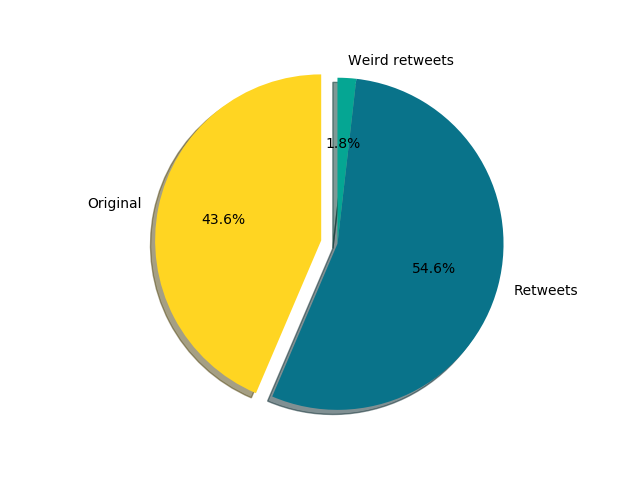
\includegraphics[width=0.6\textwidth]{C:/DATOS/MBIT/Proyecto/MBITProject_Data4all/Python/images/retweeted_proportions.png}%
\figcaption{Proporción de tuits originales y retuiteados.}
\label{fig:tuits_originales_y_retuiteados} }

\subsubsection{Número de retuits por tuit}
A la vista del gráfico anterior, parece que la actividad principal que hemos captado es
una actividad de difusión, en la que los usuarios retuitean información de otros usuarios.
Entre estos tuits retuiteados, nos interesa estudiar el número de veces que 
cada tuit ha sido retuiteado. Nos vamos a fijar en aquellos tuits que aparecen como retuiteados en nuestra muestra, es decir, aquellos tuits cuya información viene en los campos \lq\lq retweeted\_status\rq\rq o \lq\lq quoted\_status\rq\rq,
ya que son indicativos de los temas que interesan a los usuarios.
En los $8.048$ tuits de nuestro corpus que son retuits con info de lo retuiteado, se han retuiteado $2.686$ tuits distintos. La distribución del número de retuits por cada uno de estos $2.686$ aparece en las siguientes
gráficas.

\myfigure{
\begin{tabular}{cc}
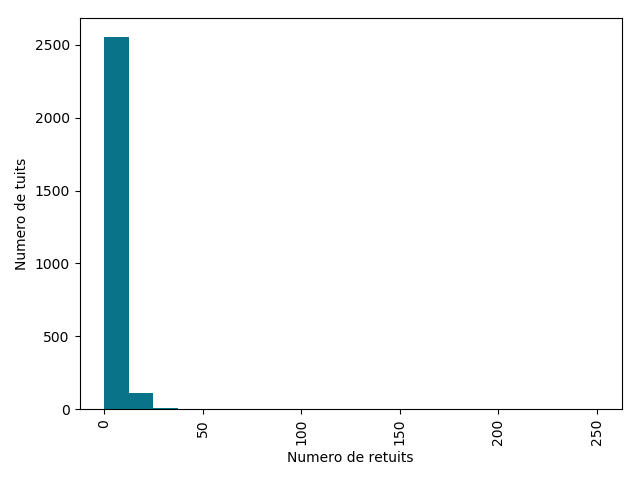
\includegraphics[width=0.4\textwidth]{C:/DATOS/MBIT/Proyecto/MBITProject_Data4all/Python/images/retweeted_graph_hist.png}
&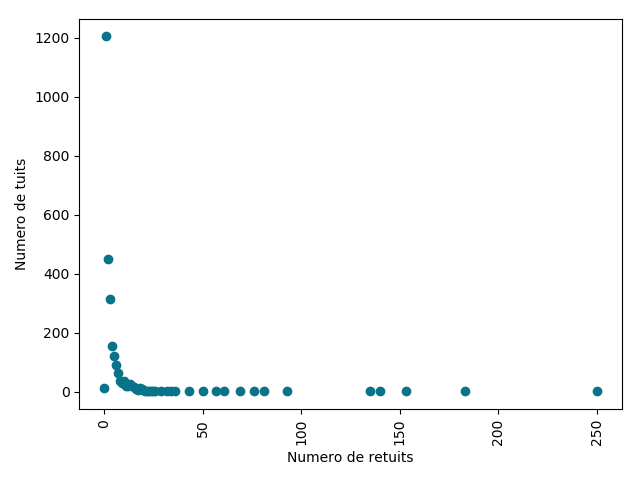
\includegraphics[width=0.4\textwidth]{C:/DATOS/MBIT/Proyecto/MBITProject_Data4all/Python/images/retweeted_graph_scatter.png}
\end{tabular}
\figcaption{Retuits: número de retuits por tuit.}
\label{fig:numero_retuits_por_tuit} }

Tanto en el histograma con en el gráfico de puntos, es claro que la mayoría de tuits han sido retuiteados unas pocas
veces (entre 1 y 5), y que solo unos pocos han sido retuiteados muchas veces. Los dos más tuiteados aparecen en la siguiente figura:

\myfigure{
\begin{tabular}{cc}

\includegraphics[width=0.4\textwidth]{tuit_mas_retuiteado}
&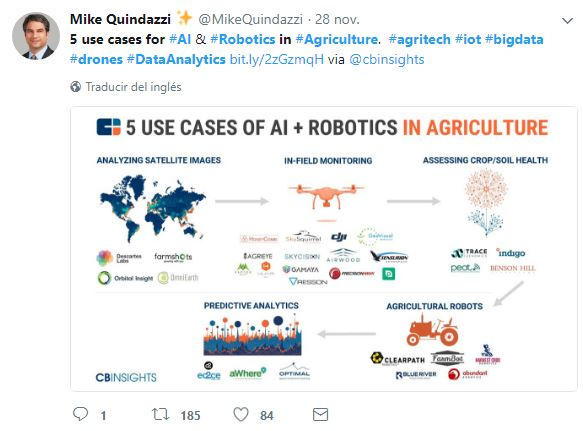
\includegraphics[width=0.4\textwidth]{tuit_mas_retuiteado2}
\end{tabular}
\figcaption{Retuits: los dos tuits más retuiteados.}
\label{fig:tuit_mas_tuiteado} }

Viendo los tuits, parece que podemos encontrar usuarios relevantes para nuestro proyecto no solo en los usuarios que han publicado los tuits que hemos descargado, sino también en los usuarios que han publicado los tuits que los primeros han retuiteado.

\subsubsection{Tuits descargados a lo largo del tiempo}
Hemos descargado tuits durante dos semanas a finales de Noviembre de 2017. La distribución
temporal del número de tuits obtenidos es la siguiente:

\myfigure{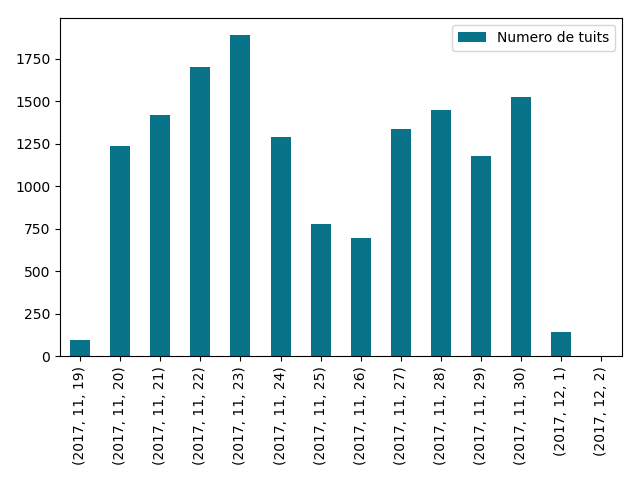
\includegraphics[width=0.6\textwidth]{C:/DATOS/MBIT/Proyecto/MBITProject_Data4all/Python/images/time_histogram.png}%
\figcaption{Tuits descargados diariamente.}
\label{fig:tuits_descargados_diariamente}}

El día 19 de Noviembre fue domingo, parece por tanto que se aprecia cierto patrón estacional en la actividad
(tuiteándose más entresemana que en fin de semana). Los días 22 y 23 de Noviembre hubo un evento
BigData, el V Encuentro de Big Data en Castilla y León, que tal vez tenga relación con la mayor actividad durante esos días.

\subsubsection{Relación entre número de tuits descargados y número de usuarios distintos}
Para nuestro proyecto, lo más relevante de la base de datos con la que trabajamos es
qué información sobre los usuarios podemos extraer a partir de los tuits almacenados. El primer paso suele ser contar, y por ello miramos cuántos usuarios distintos podemos obtener de ella. 
El siguiente gráfico representa el número de usuarios distintos en función del número de tuits
descargados, a lo largo del tiempo.

\myfigure{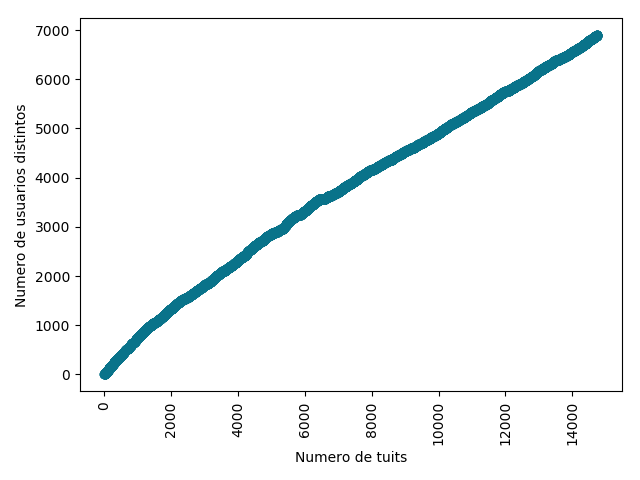
\includegraphics[width=0.6\textwidth]{C:/DATOS/MBIT/Proyecto/MBITProject_Data4all/Python/images/tuits_users_graph.png}%
\figcaption{Número de usuarios distintos frente a número de tuits descargados diariamente.}
\label{fig:tuits_users_graph}}

Este gráfico no presenta sorpresas, y se aprecia que la relación entre el número de tuits descargados y el número de usuarios distintos es prácticamente lineal.

Tenemos $6.890$ usuarios distintos (en los usuarios de los tuits descargados, sin contar los usuarios de los tuits que estos usuarios hayan podido retuitear), lo que arroja una media de unos $2.13$ tuits por usuario. Ya sabemos que la media es una medida muy poco robusta. Si queremos hacernos una idea de la actividad de nuestros usuarios, mejor estudiamos un poco más la distribución de esa variable.

\subsubsection{Número de tuits por usuario}
Al igual que hicimos con el número de retuits por tuit retuiteado, veamos un poco más en detalle
la distribución del número de tuits que cada usuario ha publicado:

\myfigure{
\begin{tabular}{cc}
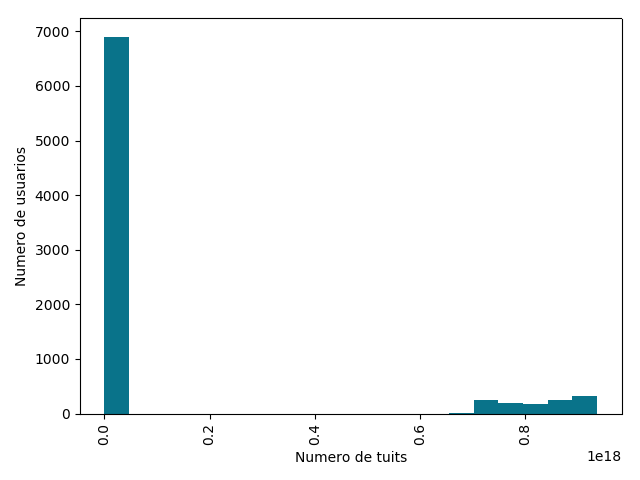
\includegraphics[width=0.4\textwidth]{C:/DATOS/MBIT/Proyecto/MBITProject_Data4all/Python/images/tuits_by_user_graph.png}
&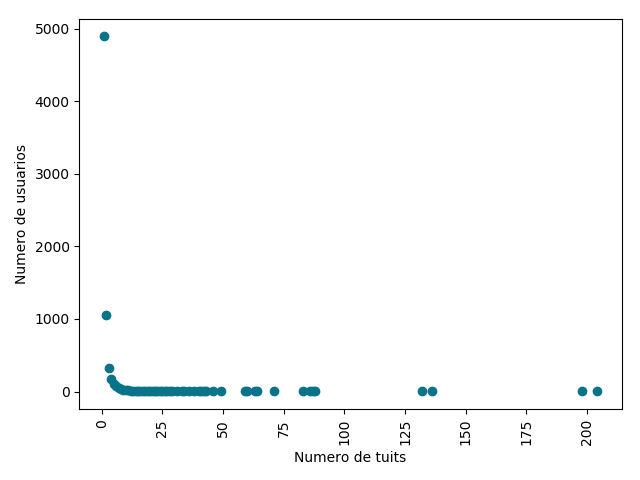
\includegraphics[width=0.4\textwidth]{C:/DATOS/MBIT/Proyecto/MBITProject_Data4all/Python/images/tuits_by_user_graph_scatter.png}
\end{tabular}
\figcaption{Número de tuits por usuario.}
\label{fig:tuits_by_user_graph_scatter} }

También en este caso se aprecia que la mayoría de los usuarios han tuiteado una vez, pero que hay algunos usuarios con un número muy elevado de tuits:

\myfigure{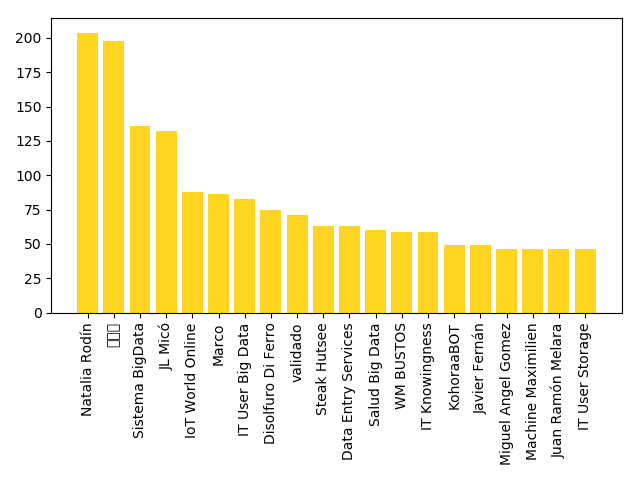
\includegraphics[width=0.6\textwidth]{C:/DATOS/MBIT/Proyecto/MBITProject_Data4all/Python/images/tuits_by_user_graph_bargraph.png}%
\figcaption{Número de tuits de los usuarios más activos.}
\label{fig:tuits_by_user_graph_bargraph}}

De estos usuarios:
\begin{itemize}
\setlength\itemsep{-0.1cm}
\item Natalia Rodín, Sistema BigData, Steak Hutsee parece que ya no existen en Twitter
\item IoT World Online es un grupo de personas interesadas en el mundo del Big Data.
\item IT User Big Data, validado, Data Entry Services, IT User Storage no está claro si son personas (solo retuits, sin bio o con bio poco descriptiva).
\item Salud Big Data es un portal de noticias
\item IT Knowingness es un feed 
\item KohoraaBot, Machine Maximilien son bots
\end{itemize}

En resumen, solo ocho de los veinte usuarios con mayor actividad parecen adecuados para
nuestro proyecto. Esto es indicativo de que la labor de filtrado de la base de datos
va a ser clave para conseguir un producto exitoso.

\subsubsection{Localización de los tuits}
Desde el punto de vista de la comercialización del producto, parece relevante incorporar información geográfica acerca de los candidatos. Para ello, siguiendo el enfoque de este trabajo, deberíamos usar información de este tipo extraída del corpus de tuits descargados de Twitter. Esto nos lleva a preguntarnos cuántos de ellos tienen el dato disponible. 

Según la documentación del API de Twitter\footnote{\url{https://developer.twitter.com/en/docs/tweets/data-dictionary/overview/geo-objects }},
los tuits pueden asociarse con una localización, generando un tuit que ha sido \lq\lq geolocalizado\rq\rq, y estas localizaciones pueden ser un punto exacto (con coordinadas de longitud y latitud) o un lugar como una ciudad o país o un área definida mediante una \lq\lq bounding box\rq\rq. Hay dos campos en un tuit que se usan para describir la geolocalización: \lq\lq coordinates\rq\rq y \lq\lq place\rq\rq. El objeto \lq\lq place\rq\rq siempre está presente en el caso de que el tuit esté geolocalizado, mientras que las coordinadas solo en el caso en el que el tuit tenga asignada una localización exacta. En el siguiente gráfico hemos 
representado el porcentaje de tuits con el campo \lq\lq place\rq\rq con valores, en el que
podemos apreciar que, salvo que cambiásemos la búsqueda en Twitter, no es un campo que vayamos a poder usar en el análisis:

\myfigure{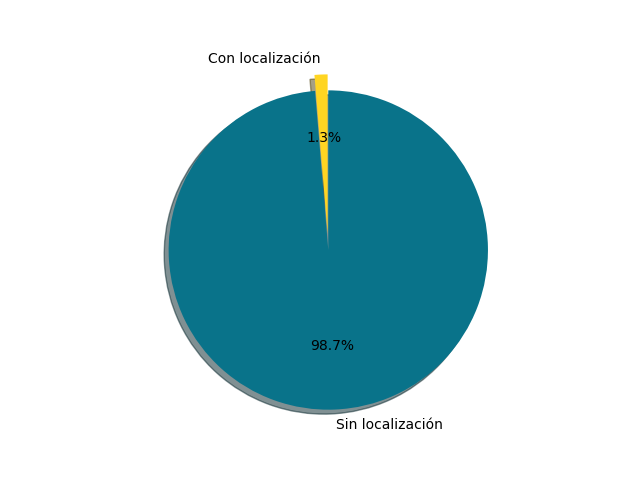
\includegraphics[width=0.6\textwidth]{C:/DATOS/MBIT/Proyecto/MBITProject_Data4all/Python/images/geolocalized_proportions.png}%
\figcaption{Proporción de tuits geolocalizados.}
\label{fig:geolocalized_proportions}}



\subsubsection{Hashtags: distribución}
En nuestro proyecto, va a ser muy importante cómo clasifiquemos los contenidos de los tuits. 
Los propios usuarios clasifican los contenidos de los tuits cuando los etiquetan a través
de los denominados \lq\lq hashtags\rq\rq,  que son palabras precedidas por el símbolo \# 
(almohadilla o {\em hash}).

Hemos estudiado los hashtags incluidos en los tuits de la base de datos, tanto los de los tuits
descargados, como de aquellos citados o retuiteados en ellos. Los siguientes gráficos dan una idea de los hashtags presentes en ambos casos:

\myfigure{
\begin{tabular}{c}
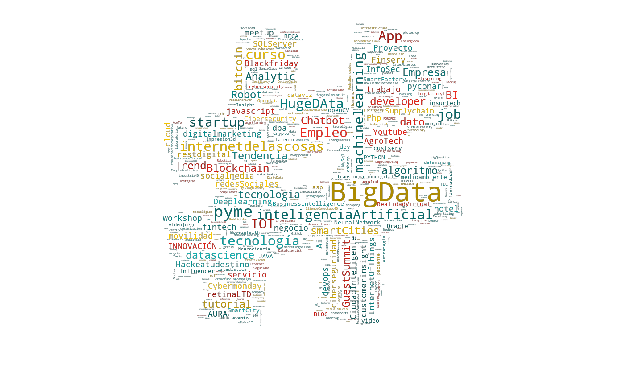
\includegraphics[width=\textwidth]{C:/DATOS/MBIT/Proyecto/MBITProject_Data4all/Python/images/hashtags_host_wordcloud.png}\\
\vspace{-1cm}\\
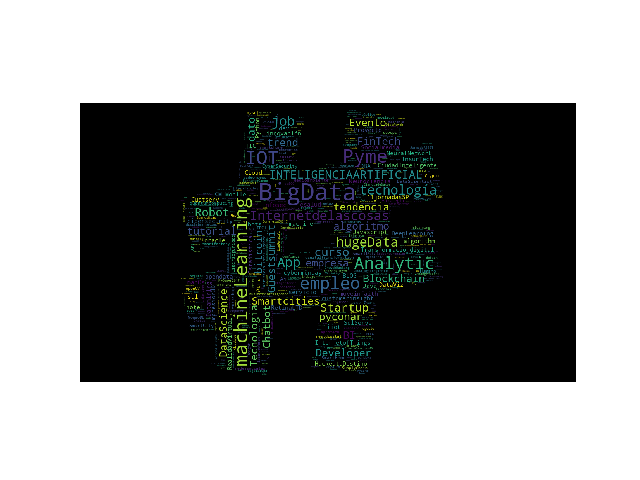
\includegraphics[width=\textwidth]{C:/DATOS/MBIT/Proyecto/MBITProject_Data4all/Python/images/hashtags_total_wordcloud.png}\\
\end{tabular}
\figcaption{Hashtags en los tuits descargados (arriba) y en los tuits descargados y citados y retuiteados en ellos.}
\label{fig:hashtags_wordcloud} }

En principio parece que no difieren mucho. Vamos a comparar los hashtags más frecuentes
en ambos conjuntos de tuits:

\myfigure{
\begin{tabular}{cc}
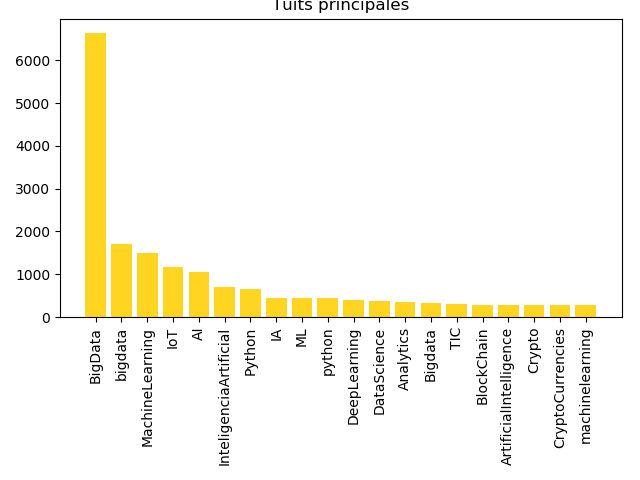
\includegraphics[width=0.4\textwidth]{C:/DATOS/MBIT/Proyecto/MBITProject_Data4all/Python/images/hashtags_host_occurs.png}
&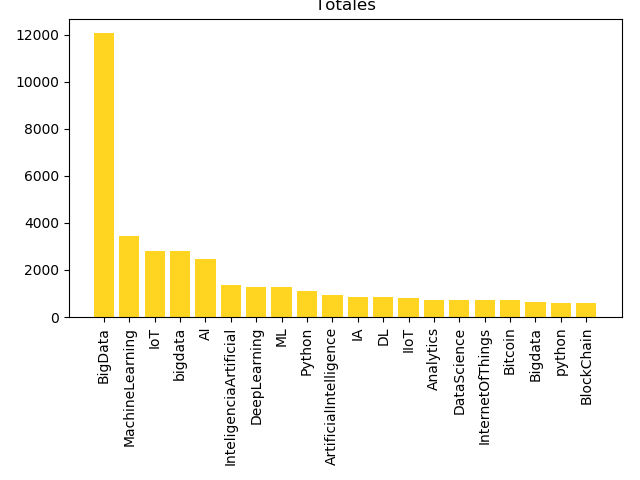
\includegraphics[width=0.4\textwidth]{C:/DATOS/MBIT/Proyecto/MBITProject_Data4all/Python/images/hashtags_total_occurs.png}
\end{tabular}
\figcaption{Hashtags más frecuentes en los tuits descargados (izq.) y en los tuits descargados y citados y retuiteados en ellos.}
\label{fig:hashtags_occurs} }

\subsubsection{Perfiles de los usuarios}
A la hora de desarrollar el proyecto y construir la lista de usuarios recomendados, es importante
filtrar aquellos que sean efectivamente personas, y desechar aquellos que sean empresas, bots, cuentas
oficiales de organismos públicos, etc.

Este análisis lo llevaremos a cabo usando la información contenida en el campo \lq\lq user\rq\rq
de los tuits, y será necesario para ello examinar el texto de la bio que incorpora, campo que
registra la información que los propios usuarios facilitan sobre ellos mismos. 
Para hacernos una idea del tipo de texto y contenidos a los que nos enfrentamos, hemos dibujado también
una nube de palabras que represente esta información.


\myfigure{
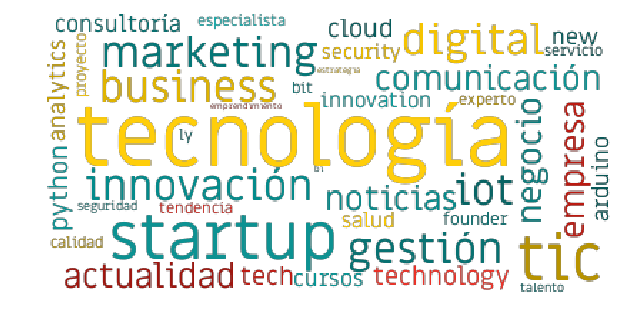
\includegraphics[width=\textwidth]{C:/DATOS/MBIT/Proyecto/MBITProject_Data4all/Python/images/bios_worldcloud2.png}
\figcaption{Wordcloud de las descripciones de los usuarios.}
\label{fig:bios_worldcloud2} }

\myfigure{
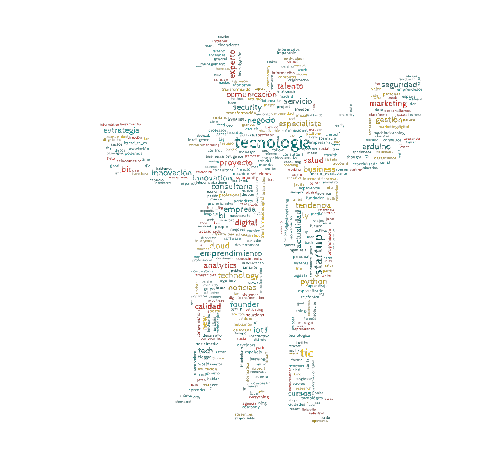
\includegraphics[width=\textwidth]{C:/DATOS/MBIT/Proyecto/MBITProject_Data4all/Python/images/bios_worldcloud.png}
\figcaption{Wordcloud de las descripciones de los usuarios.}
\label{fig:bios_worldcloud}}

Aparentemente, las descripciones de los usuarios coinciden con los perfiles que nos interesan.

\subsubsection{Origen de los tuits}
Otro elemento que nos va a proporcionar información relevante para nuestro objetivo
es la aplicación de origen del tuit. Un tuit emitido desde un dispositivo móvil es muy
probable que haya sido emitido por una persona y no por un bot o una empresa. 
Entre los campos del tuit, hay uno que refleja esta información: \lq\lq source\rq\rq\footnote{
\url{https://developer.twitter.com/en/docs/tweets/data-dictionary/overview/tweet-object }}.
Este campo describe la utilidad empleada para publicar el tuit y 
está consignada en formato HTML. Los tuits publicados desde la web
de la aplicación tienen un valor en el campo \lq\lq web\rq\rq.

A continuación describimos los principales orígenes de los tuits almacenados en 
nuestra base de datos, y al igual que con los hashtags, comparamos los de los tuits
descargados, y los de aquellos citados o retuiteados en ellos:

\myfigure{
\begin{tabular}{cc}
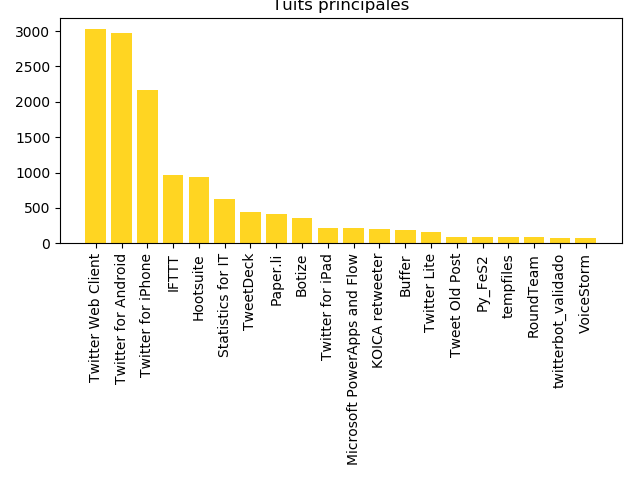
\includegraphics[width=0.4\textwidth]{C:/DATOS/MBIT/Proyecto/MBITProject_Data4all/Python/images/sources_host.png}
&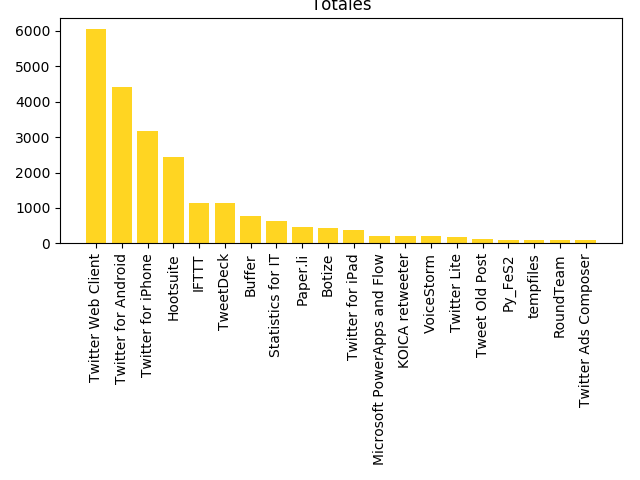
\includegraphics[width=0.4\textwidth]{C:/DATOS/MBIT/Proyecto/MBITProject_Data4all/Python/images/sources_total.png}
\end{tabular}
\figcaption{Orígenes más frecuentes en los tuits descargados (izq.) y en los tuits descargados y citados y retuiteados en ellos.}
\label{fig:sources} }

Estos orígenes quieren decir:
\begin{itemize}
\item Twitter web client: son tuits producidos desde la página web de Twitter
\item Twitter for Android, Twitter for iPhone, Twitter for iPad: tuits enviados desde las aplicaciones
de Twitter para los sistemas operativos de los dispositivos móviles.
\item IFTTT, Hootsuite, Paper.li, RoundTeam: son herramientas que sirven para gestionar 
la actividad en plataformas
sociales, por ejemplo publicar automáticamente contenidos (Twitter entre otras).
\item Statistics for IT, Koica retweeter: parecen retuits automáticos por parte
de alguna organización.
\item TweetDeck es una herramienta oficial creada por Twitter para gestionar y controlar 
varias cuentas desde un solo lugar. Se pueden controlar notificaciones, menciones, 
mensajes y la actividad en general de una o varias cuentas, y por supuesto programar envíos
de tuits.
\item Botize es una herramienta para automatizar tareas, en particular en Twitter. 
Los tuits con este origen serán probablemente de bots.
\item PowerApps and Flow: PowerApps es un servicio de Microsoft 
orientado fundamentalmente a empresas para crear aplicaciones. Microsoft Flow 
es un servicio también enfocado sobre todo a empresas, para principalmente ayudarles a 
automatizar tareas entre sus sistemas y algunos de terceros (Twitter entre ellos).
\item Twitter Lite: es una versión oficial de Twitter, enfocada sobre todo a usuarios 
de países emergentes, que funciona a través del explorador y que minimiza el uso de datos 
y mejora la velocidad de carga en conexiones lentas.
\item Tweet Old Post: es un plugin de WordPress, que retuitea de forma aleatoria y 
automática entradas antiguas de un blog alojado en dicha plataforma.
\item Buffer, Py\_FeS2, tempfiles, twitterbot\_validado: no está muy claro lo que representan. 
En Twitter, @Py\_FeS2 es un usuario nuevo, de Noviembre de 2017, que por el volumen 
tuiteado parece un bot.
\item VoiceStorm: es una aplicación que permite a los empleados de una empresa
promocionar la entidad en la que trabajan a través de las redes sociales.
\end{itemize}

De este análisis parece que si un tuit proviene de un origen como Twitter web client,
Twitter for Android, Twitter for iPhone, Twitter for iPad, Twitter Lite, Tweet Old Post
y VoiceStorm, es bastante probable que el usuario sea una persona (y por tanto un posible
usuario relevante para el objetivo del proyecto). A continuación mostramos
los tuits clasificados como \lq\lq posibles personas\rq\rq y \lq\lq posibles otros\rq\rq
atendiendo a este criterio:

\myfigure{
\begin{tabular}{cc}
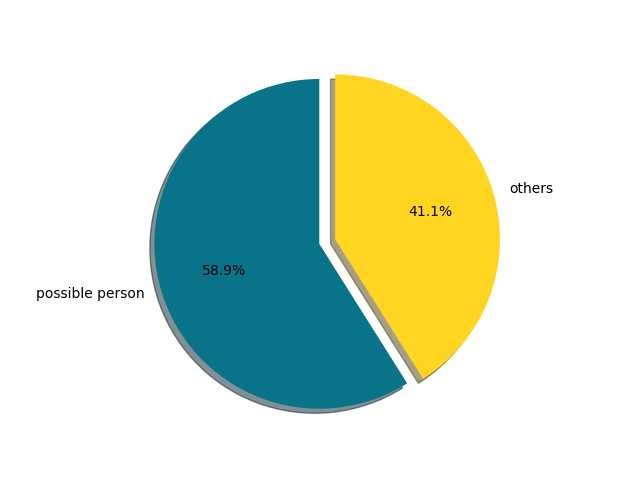
\includegraphics[width=0.4\textwidth]{C:/DATOS/MBIT/Proyecto/MBITProject_Data4all/Python/images/sources_people_percentage_host.png}
&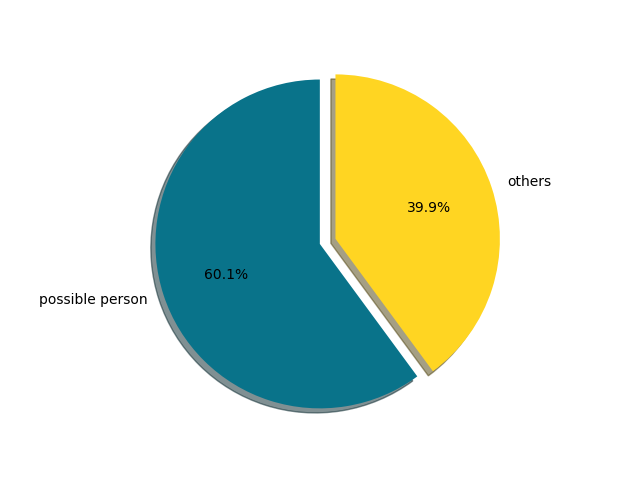
\includegraphics[width=0.4\textwidth]{C:/DATOS/MBIT/Proyecto/MBITProject_Data4all/Python/images/sources_people_percentage_total.png}
\end{tabular}
\figcaption{Porcentaje en los datos de los tuits cuyo origen indican posibles personas en 
los tuits descargados (izq.) y en los tuits descargados y citados y retuiteados en ellos.}
\label{fig:sources_percentage} }